\chapter{Members' Summary Report}
\label{chap:members_summary_report}
\lhead{Chapter 7. Members' Summary Report}

This chapter provides a detailed summary of the contributions of each team member throughout the project lifecycle. It outlines their primary roles, responsibilities, and key achievements in ensuring the quality and success of the Library Management System.

\section{Tishko Salah Hawez (Test Manager)}
\label{sec:tishko_salah_summary}
\textbf{ID:} 02-24-00022

\subsection{Overview of Role and Responsibilities}
As the Test Manager, Tishko Salah Hawez was entrusted with the overall responsibility for the project's testing and quality assurance strategy. His role was central to ensuring that the Library Management System met the functional, non-functional, and quality requirements outlined in the Software Requirements Specification (SRS). He was responsible for the entire testing lifecycle, from initial planning and strategy formulation to the management of test execution, defect tracking, and final reporting.

His leadership ensured a structured and comprehensive testing process, coordinating the efforts of the entire team to validate the application's stability, reliability, and usability. He was the primary driver behind the creation and maintenance of the formal Test Plan (detailed in Chapter 3), which served as the guiding document for all testing activities.

\subsection{Test Planning and Strategy}
Tishko's primary contribution began with the development of a comprehensive test strategy. He meticulously analyzed the SRS to define the scope of testing, identify key user roles (Librarian, Member), and map out critical use cases such as user authentication, book management, and borrowal processing.

Key activities in this phase included:
\begin{itemize}
    \item \textbf{Scope Definition:} Establishing clear boundaries for what would be tested, focusing on the core functionalities defined in the SRS and prioritizing tests based on risk and user impact.
    \item \textbf{Test Scheduling:} Creating and managing the project's testing timeline, as visualized in the Gantt chart in Chapter 3, to ensure that testing milestones were aligned with development progress.
    \item \textbf{Resource Allocation:} Assigning testing tasks to team members based on their roles (Coders vs. Non-Coders) and expertise, as defined in the project's responsibility matrix (\texttt{Tasks.tex}).
    \item \textbf{Tool Selection:} Leading the evaluation and selection of appropriate testing frameworks and tools, including Jest for unit testing, Cypress for end-to-end testing, and Postman for API testing.
\end{itemize}

\subsection{Execution Management and Coordination}
Tishko actively supervised and coordinated the execution of all testing levels and types. He ensured that the test cases designed by the team were robust, comprehensive, and directly traceable to the requirements. His oversight was critical across the following testing domains:
\begin{itemize}
    \item \textbf{Functional and API Testing:} He led the non-coding team members in designing and executing black-box test cases for all major features, including entity management, authentication, and state transitions. He also oversaw the manual verification of API endpoints to ensure data integrity and correct error handling.
    \item \textbf{Unit and Integration Testing:} While developers were responsible for writing unit tests, Tishko reviewed the results and coverage reports to ensure that critical components were adequately tested at a code level. He guided the strategy for integration testing to verify seamless data flow between the frontend and backend.
    \item \textbf{Non-Functional Testing:} He managed the execution of usability, security, performance, and browser compatibility tests to ensure the application was not only functional but also user-friendly, secure, and performant under various conditions.
    \item \textbf{Regression and Deployment Testing:} After each new build or bug fix, Tishko coordinated the execution of regression test suites to prevent new changes from breaking existing functionality. He also managed the smoke and acceptance testing following deployment to ensure the stability of the live environment.
\end{itemize}

\subsection{Reporting, Defect Management, and Quality Assurance}
A core part of Tishko's role was monitoring testing progress and reporting on the quality of the application. He established a systematic process for defect management, where bugs were documented, prioritized, assigned, and tracked through to resolution.

He utilized the dashboards and reports generated by the testing tools to provide clear visibility into the project's health. For instance, he used the Cypress Dashboard to monitor end-to-end test runs and Jest coverage reports to assess the thoroughness of unit tests.

\begin{figure}[H]
    \centering
    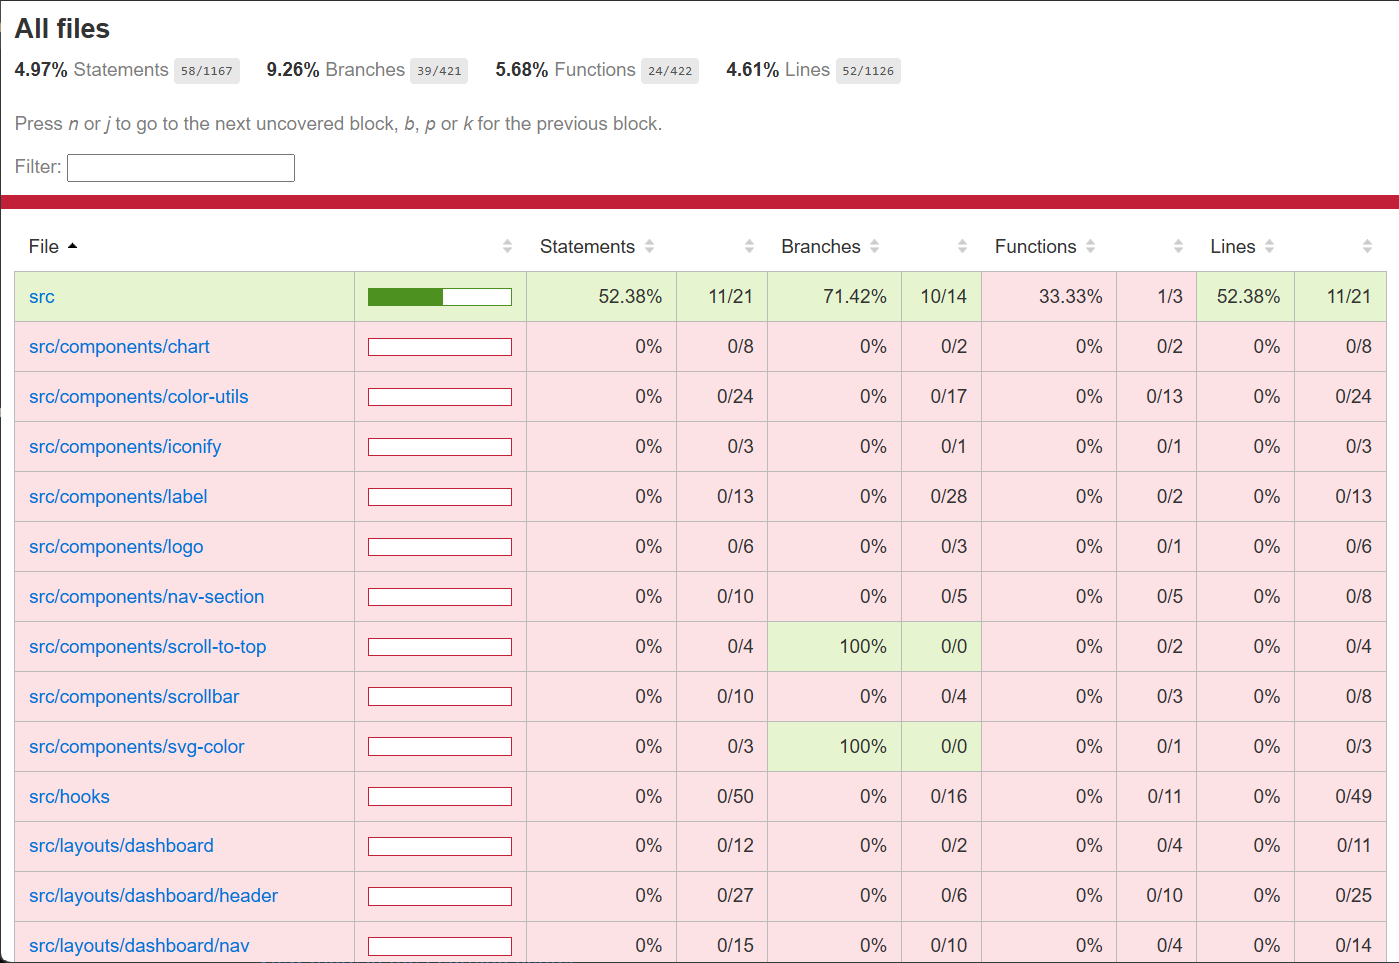
\includegraphics[width=0.8\textwidth]{assets/jest/coverage_test_report_jest_frontend.png}
    \caption{Frontend Test Coverage Report Overseen by the Test Manager.}
    \label{fig:tishko_jest_report}
\end{figure}

\begin{figure}[H]
    \centering
    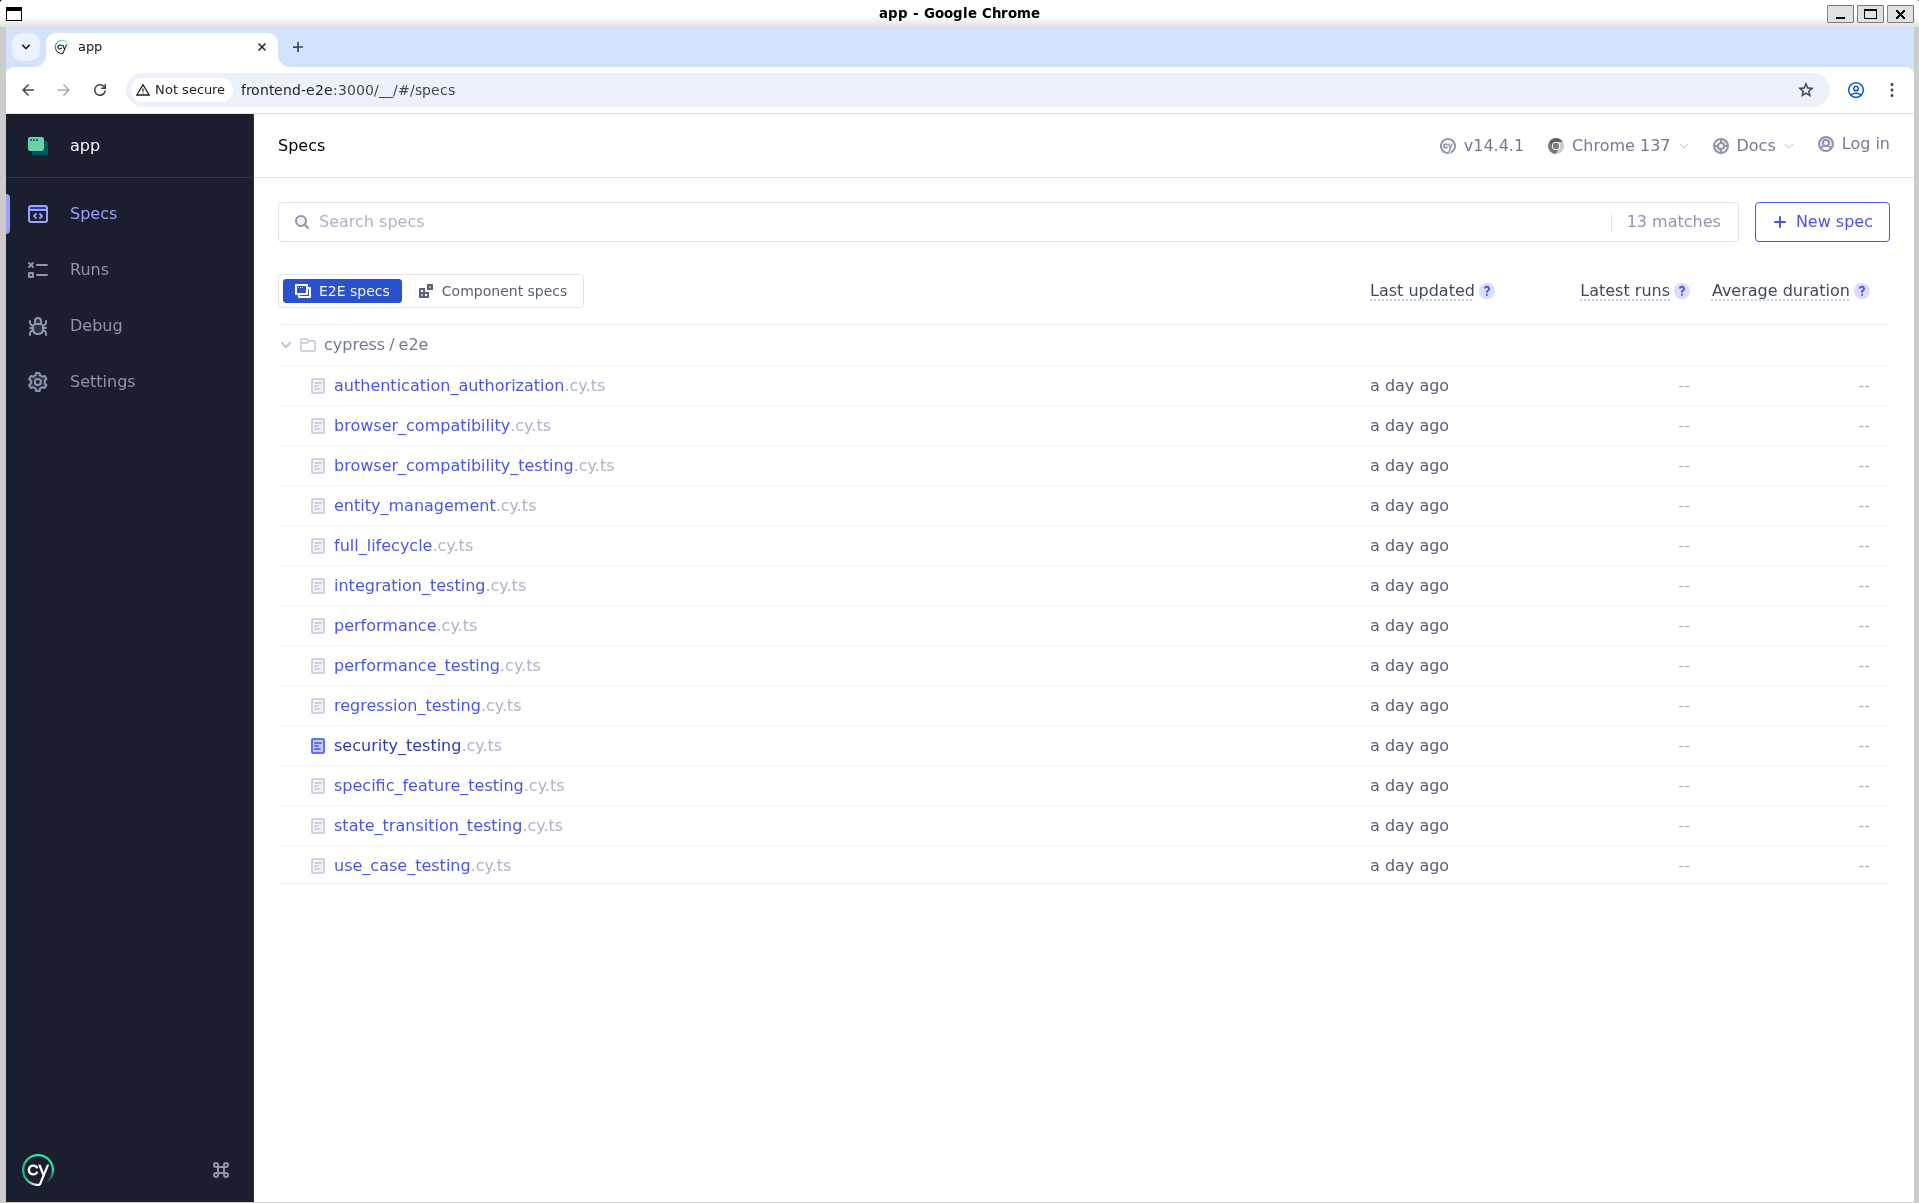
\includegraphics[width=0.8\textwidth]{assets/cypress_dashboard.png}
    \caption{Cypress Dashboard for E2E Test Run Monitoring.}
    \label{fig:tishko_cypress_dashboard}
\end{figure}

\subsection{Documentation and Static Testing}
Beyond dynamic testing, Tishko championed the importance of static testing. He led the review of all critical project documents, including the SRS, Test Plan, and individual test case documents, to ensure they were clear, accurate, and complete. This proactive approach helped identify ambiguities and inconsistencies early in the lifecycle, preventing potential defects. His diligence was instrumental in compiling the testing-related chapters of this final report.

\subsection{Conclusion}
Tishko Salah Hawez's performance as Test Manager was fundamental to the successful delivery of a high-quality Library Management System. His systematic approach to test planning, rigorous oversight of execution, and clear-sighted reporting ensured that the project adhered to its quality objectives. His leadership fostered a culture of quality within the team and was directly responsible for the identification and resolution of numerous defects, ultimately leading to a more stable and reliable product.

